\section{Introduction}

Pour mon stage de fin de licence, j'avais le choix entre un stage de 7~semaines en entreprise ou en laboratoire, selon que je souhaitais m'orienter vers le monde professionnel ou académique. Étant donné que je veux me diriger vers une carrière professionnelle, j'ai choisi d'effectuer mon stage en entreprise chez Orano.
\subsection{Orano}
Orano est un grand groupe français spécialisé dans le cycle du nucléaire. Il compte 17~500~collaborateurs repartis dans 17~pays et avait un chiffre d'affaire de 4,8~M€ en 2023~\cite{report:rapport_activiter}. Né en 2018 à la suite d'une restructuration d'Areva, il est présent dans l'ensmeble du cycle du combustible nucléaire, de l'extraction de l'uranium à la gestion des déchets nucléaires en passant par la production de combustible. Ses différentes activités sont réparties dans plusieurs business units~:
\begin{description}
    \item [Orano Support]  regroupe les activités de support du groupe.
    \item [Orano Mining] regroupe les activités d'extraction d'uranium.
    \item [Orano Medical] regroupe les activités de production de radioéléments pour la médecine nucléaire.
    \item [Orano Batteries] regroupe les activités de recyclage de batterie.
    \item [Orano Dismantling] regroupe les activités de démantèlement de centrale nucléaire.
    \item [Orano Chimie-Enrichissement] regroupe les activités de chimie et d'enrichissement de l'uranium.
\end{description}
\begin{figure}[hb]
    \centering
    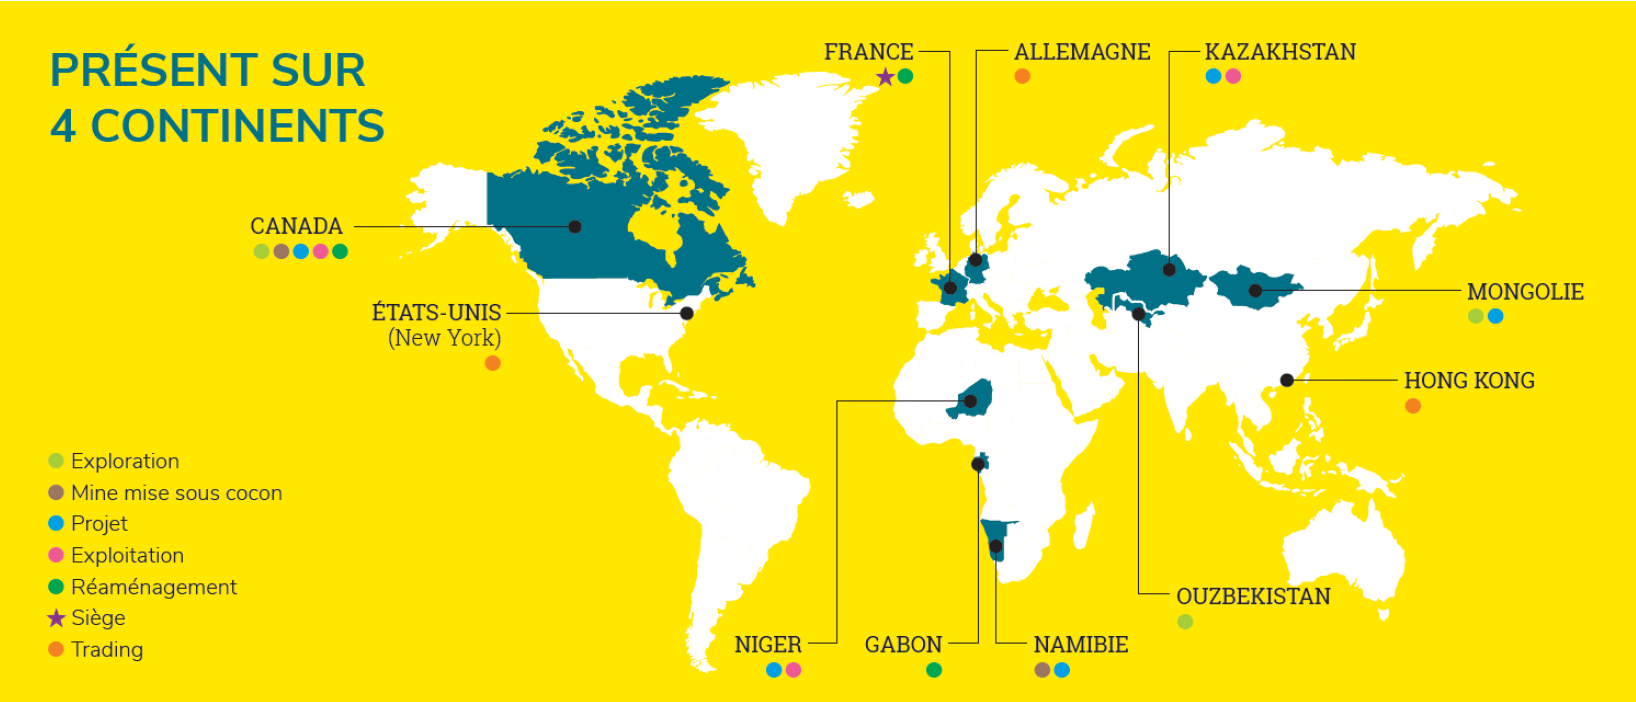
\includegraphics[width=\textwidth]{Carte-ornao-international.png}
    \caption[Carte des activités d’Orano dans le monde]{Carte des activités d’Orano dans le monde, Source~: Dossier d’information Orano~2020}
    \label{fig_carte_orano}
\end{figure}




\subsection{Orano Mining}

En ce qui conerne Ornao Mining, Ces filiales sont présentes à l'international avec des mines d'uranium au Kazakhstan, au Canada et au Niger, ainsi que des explorations ou des projets en Namibie, en Ouzbékistan et en Mongolie. La majorité des sites à l'étranger d'Orano sont des sites d'Orano Mining en raison de la nature de ses activités. C'est dans cette dernière que j'ai effectué mon stage.

Orano mining est en charge de tout ce qui est relatif à l'extraction de l'uranium. Ces activités sont reparties en 5~grands domaines~:%remediation generation de nouveux projet et exploration. explo ,prod, projet, remediation (amf) %parler de nouveaux projet

\subsubsection{La génération de nouveaux projets}
La mine mène de nombreux projets qui peuvent prendre diverses formes. Cela va de la création de petits projets comme de nouveaux outils à la recherche de nouveaux gisements et la création des infrastructures pour les exploiter. Par exemple, Orano a créé une usine de traitement au Kazakhstan ainsi qu'une base de vie associée. En Namibie, Orano a créé une usine de dessalage pour subvenir aux besoins en eau de la future mine de Trekkopje.

\subsubsection{L'exploration}
L'exploration est la première étape de l'extraction de l'uranium. Elle consiste à trouver des gisements d'uranium. Pour cela, Orano Mining utilise des méthodes géophysiques et géochimiques pour trouver des gisements d'uranium. Une fois un gisement trouvé, il faut l'exploiter.

\subsubsection{L'exploitation}
L'exploitation est la deuxième étape de l'extraction de l'uranium. Elle consiste à extraire l'uranium du sol. Pour cela, Orano Mining utilise diverses méthodes d'extraction en fonction de la nature du gisement. On peut citer~:
\begin{description}

    \item [L'extraction à ciel ouvert]qui consiste à creuser une fosse pour extraire l'uranium. C'est le cas de la mine de Somaïr au Niger et de Mclean Lake au Canada (production suspendue entre 2008 et 2025 suite à la chute du cours de l'uranium).
    \item [L'extraction in situ] qui consiste à injecter de l'acide dans le sol entre deux couches étanches pour dissoudre l'uranium et le remonter à la surface. C'est le cas des mines de Muyunkum et Tortkuduk au Kazakhstan.
    \item [L'extraction par jetboring]qui consiste à creuser un trou dans le sol et à injecter de l'eau sous pression pour remonter l'uranium à la surface. C'est le cas de la mine Cigar Lake au Canada.

\end{description}

\subsubsection{Le traitement}


Le traitement est la dernière étape de l'extraction de l'uranium. Elle consiste à traiter le minerai pour en extraire l'uranium. Pour cela, Orano Mining utilise des méthodes de traitement chimique pour extraire l'uranium du minerai. Généralement, cette étape est faite avec une lixiviation de l'uranium par une solution concentrée acidique, alcaline ou de peroxyde pour former ce que l'on appellera du "yellow cake" due à sa couleur et texture (voir \cref{fig_yellow-cake}). Le yellow cake est composé de 70~\% à 90~\% d'oxyde d'uranium notamment d'$U_3O_8$~\cite{article:composition-yellow-cake}. Une fois l'uranium extrait, il est envoyé à Orano Chimie-Enrichissement ou à d'autres partenaires pour être enrichi. En effet, l'uranium naturel est composé à 0,7~\% d'uranium~235 et à 99,3~\% d'uranium~238 avec une concentration moyenne de 2,7~ppm~\cite{site:natural_uranium}. Pour être utilisé dans un réacteur, il faut que l'uranium~235 soit enrichi entre 3~\% à 5~\% d'$U_{238}$~\cite{article:uranium-concentration}



\subsubsection{L'après-mine}
\begin{wrapfigure}{r}{0.5\textwidth}
    \centering
    \href{https://commons.wikimedia.org/wiki/File:Yellow_Cake_Uranium_(14492248719).jpg}{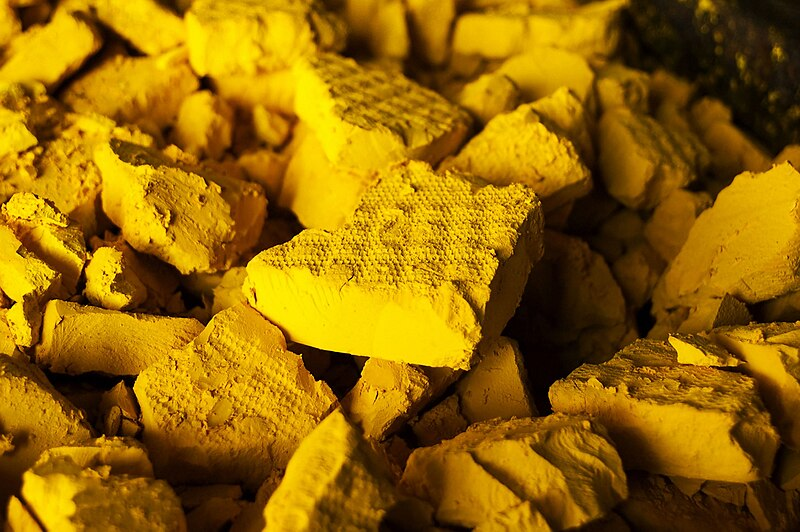
\includegraphics[width=0.5\textwidth]{Yellow_Cake_Uranium_(14492248719).jpg}}
    \caption[Apparence du yellow cake]{Apparence de yellow cake. Avec des méthodes modernes, certains traitements peuvent lui donner une apparence marron, voir noir. Source~: \href{https://commons.wikimedia.org/wiki/File:Yellow_Cake_Uranium_(14492248719).jpg}{Nuclear Regulatory Commission from US}, Public domain, via Wikimedia Commons}
    \label{fig_yellow-cake}
\end{wrapfigure}
L'après-mine désigne l'ensemble des actions de remédiation et de monitoring qui sont effectuées par Orano après qu'une mine ferme. En effet, une fois une mine fermée, il faut la remettre en état pour éviter les risques de pollution. Pour cela, Orano Mining met en place des systèmes de monitoring pour surveiller l'évolution de la mine et des actions de remédiation pour remettre la mine en état. En France, Orano a la charge de 235 sur 247 des sites miniers d'uranium présent sur le territoire dont des sites qu'Orano n'a pas exploité~\cite{site:orano_apres_mine}. L'après-mine n'intervient pas qu'en France, mais aussi a l'étranger. Par exemple, au Canada, Orano a fini la remédiation de la mine de Cluff Lake (1979-2002) en 2013 et le site a été réouvert au public. En 2023, le gouvernement a été satisfait des actions d'Orano et les terres, on était rendu à l'état provincial~\cite{site:Cluff_lake_remediation}.



\subsection{Direction de la transformation digitale}
% fait partie des projet de la mine %pas petit 
Au sein de la mine, un service de la direction des projets est responsable de la transformation digitale. C'est là que j'ai effectué mon stage. Ce service met en place divers outils digitaux pour accompagner les projets et les exploitations dans le monde numérique de demain. Il travaille en collaboration avec les différents services de la mine pour comprendre leurs besoins et mettre en place des outils qui y répondent. Voici quelques exemples de projets en cours lors de mon stage~:



\begin{itemize}
    \item La digitalisation des procédures de Katco, la joint-venture d'Orano au Kazakhstan.
    \item La numérisation et l'indexation des documents de la mine ainsi que des plans géologiques afin de les rendre plus facilement accessibles aux collaborateurs.
    \item La collecte et l'analyse de données pour trouver des solutions permettant de gagner en efficacité.
\end{itemize}


\subsection{Choix du Stage}
J'envisage plus tard de devenir ingénieur en \href{https://fr.wikipedia.org/wiki/M%C3%A9catronique}{mecatronique} et j'ai donc chercher un stage orienter en informatique, en électronique, en mécanique ou idéalement, un mix des trois. Le nucléaire est également un sujet qui m'intéresse et dont je comprends un certain nombre de choses. J'ai donc postulé chez Orano pour mon stage de fin de licence. %faire gaffe resentie perso %J'ai également la conviction que nous ne pourrons pas faire face à la catastrophe climatique qui s'annonce sans le nucléaire.
\subsection{Objectif du stage}

Orano réalise souvent des projets via la direction de la R\&D et de l'innovation pour améliorer ses activités, mais souvent il y a un manque de temps et de ressource pour revenir sur des projets déjà existants. J'ai donc été recruté pour essayer d'apporter des optimisations à un outil déjà existant: La \nameref{sec_CanOp}. Cet outil a été développé entre 2018 et 2022 et pesé environ 5kg. L'objectif du stage était de le rendre plus léger et plus robuste.